\documentclass[twoside,openright]{book}



\usepackage{amsmath}
\usepackage{verbatim}
\usepackage{graphicx}
\usepackage{hyperref}
\usepackage{fixltx2e}		%allows subscript to be used
\usepackage{float}
\usepackage{times}
\usepackage{lastpage}
\usepackage{subfig}
\usepackage{color}
\usepackage{xcolor}
\usepackage[tikz]{bclogo}
\usepackage{enumitem}
\setlist{nolistsep}

\usepackage{textcomp}

\definecolor{bgblue}{RGB}{245,243,253}
\definecolor{ttblue}{RGB}{91,194,224}
 


%set margins
%set paper dimensions
\usepackage[paperwidth=5.5in, paperheight=8.5in]{geometry}
\usepackage{emptypage}

%set header and footer
\usepackage{fancyhdr}
\pagestyle{fancy}
\fancyhead{}
\fancyfoot{}

\renewcommand{\chaptermark}[1]{\markboth{\thechapter\ |\ #1}{}}
		
		
	
\lhead{\leftmark}
\rhead{\thepage}


%set spacing
\usepackage{setspace}
\singlespacing

%CONSOLE TITLE
\definecolor{lightblue}{rgb}{0.85,1,1} 
\definecolor{lightgreen}{rgb}{0.8,1,0.9} 
\definecolor{darkblue}{rgb}{0,0,0.5} 
\definecolor{darkred}{rgb}{0.6,0,0} 




\usepackage{listings}
\usepackage{courier}

\definecolor{spin_pub}{RGB}{191,223,255}
\definecolor{spin_pri}{RGB}{191,248,255}
\definecolor{spin_con}{RGB}{191,248,255}
\definecolor{spin_dat}{RGB}{191,255,200}
\definecolor{spin_num}{RGB}{48,136,146}
\definecolor{spin_str}{RGB}{246,7,47}
\definecolor{spin_comment}{RGB}{110,110,110}
\definecolor{spin_operator}{RGB}{0,128,1}
\definecolor{spin_ctrl}{RGB}{128,128,128}

\lstdefinelanguage{Spin}{
  classoffset=0,
  morekeywords={con, var, obj, pub, pri, dat},
  morekeywords={chipver, clkmode, \_clkmode, clkfreq, \_clkfreq, clkset, \_xinfreq, \_stack, \_free, rcfast, rcslow, xinput, xtal1, xtal2, xtal3, pll1x, pll2x, pll4x, pll8x, pll16x},
  morekeywords={cogid, cognew, coginit, cogstop, reboot},
  morekeywords={locknew, lockret, lockclr, lockset, waitcnt, waitpeq, waitpne, waitvid},
  morekeywords={bytefill, wordfill, longfill, bytemove, wordmove, longmove, lookup, lookupz, lookdown, lookdownz, strsize, strcomp},
  morekeywords={string, constant, float, round, trunc, file},
  morekeywords={dira, dirb, ina, inb, outa, outb, cnt, ctra, ctrb, frqa, frqb, phsa, phsb, vcfg, vscl, par, spr},
  morekeywords={true, false, posx, negx, pi, result},
  morekeywords={org, fit, res},
  keywordstyle={\color{black} \bf},
  classoffset=1,
  morekeywords={byte, word, long},
  keywordstyle={\color{darkblue} \bf},
  classoffset=2,
  morekeywords={clkset, cogid, coginit, cogstop},
  morekeywords={locknew, lockret, lockclr, lockset, waitcnt, waitpeq, waitpne, waitvid},
  morekeywords={if\_always, if\_never, if\_e, if\_ne, if\_a, if\_b, if\_ae, if\_be, if\_c, if\_nc, if\_z, if\_nz, if\_c\_eq\_z, if\_c\_ne\_z, if\_c\_and\_z, if\_c\_and\_nz, if\_nc\_and\_z, if\_nc\_and\_nz, if\_c\_or\_z, if\_c\_or\_nz, if\_nc\_or\_z, if\_nc\_or\_nz, if\_z\_eq\_c, if\_z\_ne\_c, if\_z\_and\_c, if\_z\_and\_nc, if\_nz\_and\_c, if\_nz\_and\_nc, if\_z\_or\_c, if\_z\_or\_nc, if\_nz\_or\_c, if\_nz\_or\_nc},
  morekeywords={call, djnz, jmp, jmpret, tjnz, tjz, ret, nr, wr, wc, wz},
  morekeywords={rdbyte, rdword, rdlong, wrbyte, wrword, wrlong},
  morekeywords={abs, absneg, neg, negc, negnc, negz, negnz, min, mins, max, maxs, add, addabs, adds, addx, addsx, sub, subabs, subs, subx, subsx, sumc, sumnc, sumz, sumnz, mul, muls, and, andn, or, xor, ones, enc, rcl, rcr, rev, rol, ror, shl, shr, sar, cmp, cmps, cmpx, cmpsx, cmpsub, test, testn, mov, movs, movd, movi, muxc, muxnc, muxz, muxnz, hubop, nop},
  keywordstyle={\color{darkred} \bf},  
  classoffset=3,
  morekeywords={if, elseif, ifnot, elseifnot, else, case, other, repeat, from, to, step, until, while, next, quit, return, abort},
  keywordstyle={\color{spin_ctrl} \bf},  
  classoffset=4,
  alsoletter={+,-,=,:,\^,|,~,?,<,>,!,@,\#},
  morekeywords={+,-,--,++,\^\^,||,~,~~,?,|<,>|,!,NOT,@,@@,=,:=,+=,-=,*=,**=,*,**,/,//,/=,//=,\#>,\#>=,<\#,<\#=,~>,~>=,<<,<<=,>>,>>=,<-,<-=,->,->=,><,><=,\&,\&=,|,|=,\^,\^=,AND,AND=,OR,OR=,==,===,<>,<>=,<,<=,>,>=,=<,=<=,=>,=>=},
  keywordstyle={\color{spin_operator} \bf},  
  classoffset=0,
  morecomment=[l]{'},
  morecomment=[n]{\{}{\}},
  commentstyle=\color{spin_comment},
  numberstyle=\color{spin_num},
  sensitive=false,
  showtabs=false,
  showspaces=false,
  showstringspaces=false,
  breaklines=true,
  breakatwhitespace=true,
  basicstyle=\footnotesize\ttfamily,
  numbers=none,
  frame=single,
  framesep=0.10in,
  xleftmargin=0.10in,
  xrightmargin=0.10in,
  aboveskip=5pt,
  belowskip=5pt
}


\lstdefinestyle{C++}{
language=C++,                % choose the language of the code
basicstyle=\small,       % the size of the fonts that are used for the code
numbers=left,                   % where to put the line-numbers
numberstyle=\footnotesize,      % the size of the fonts that are used for the line-numbers
stepnumber=1,                   % the step between two line-numbers. If it's 1 each line 
numbersep=10pt,                  % how far the line-numbers are from the code
showspaces=false,               % show spaces adding particular underscores
showstringspaces=false,         % underline spaces within strings
showtabs=false,                 % show tabs within strings adding particular underscores
frame=none,	                % adds a frame around the code
tabsize=1,	                % sets default tabsize to 2 spaces
captionpos=t,                   % sets the caption-position to bottom
breaklines=true,                % sets automatic line breaking
breakatwhitespace=true,        % sets if automatic breaks should only happen at whitespace
backgroundcolor=\color{white},
keywordstyle={\color{black} \bf}
}

\lstdefinestyle{spin}{
language=Spin,
backgroundcolor=\color{spin_pub}
}


\lstdefinestyle{pasm}{
language=Spin,
backgroundcolor=\color{spin_dat}
}





\usepackage{eso-pic}
\newcommand\ChapterBackgroundPic{%
    \put(0,0){%
        \parbox[b][\paperheight]{\paperwidth}{%
            \vfill
            \centering
            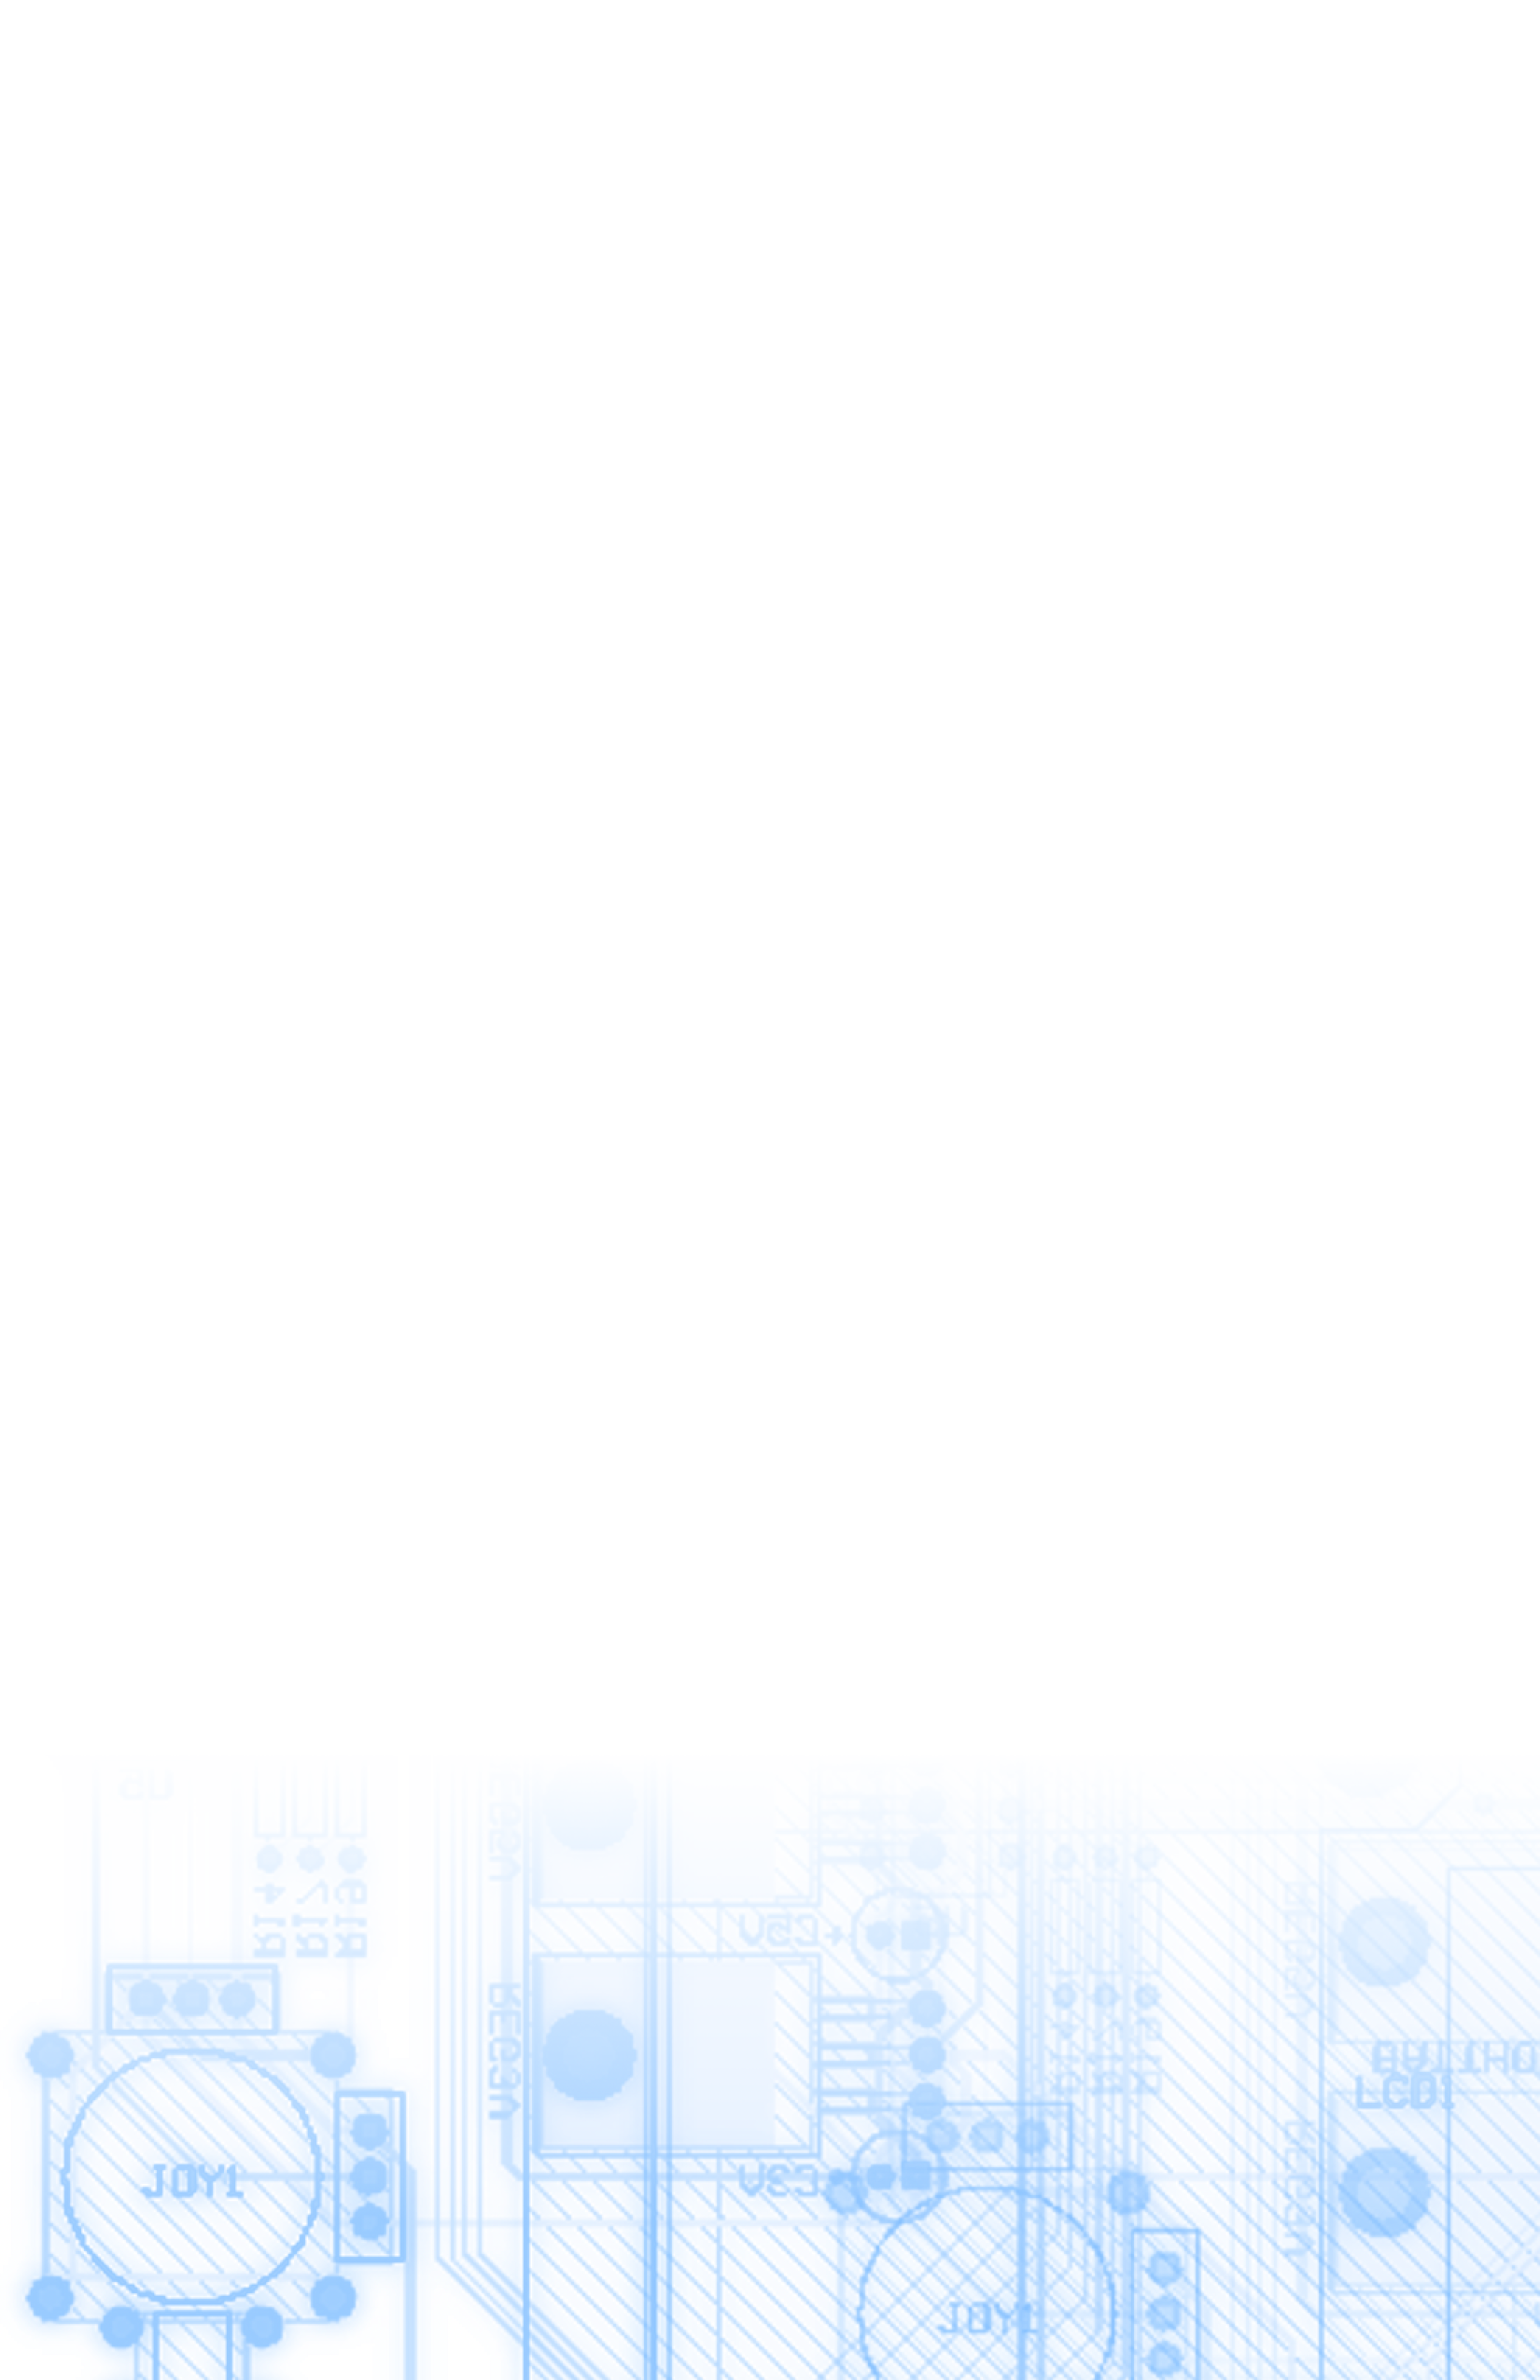
\includegraphics[width=\paperwidth,height=\paperheight,%
            keepaspectratio]{graphics/bookcover_chapter.png}%
            \vfill
}}}

\usepackage{pdfpages}


\usepackage{makeidx}

\usepackage[T1]{fontenc}
\usepackage{titlesec, blindtext, color}
\definecolor{gray75}{gray}{0.75}
\newcommand{\hsp}{\hspace{20pt}}
\titleformat{\chapter}[hang]{\Huge\bfseries}{\thechapter\hsp\textcolor{gray75}{|}\hsp}{0pt}{\Huge\bfseries}


\setcounter{secnumdepth}{1}
\setcounter{tocdepth}{1}


\title{{A Crash Course In LameStation} \\ Digital Synthesis, Computer Architecture, and Electronics Design Explored}
\date{}
\author{Brett Weir}



\begin{document}

\lstset{style=C++}

\frontmatter

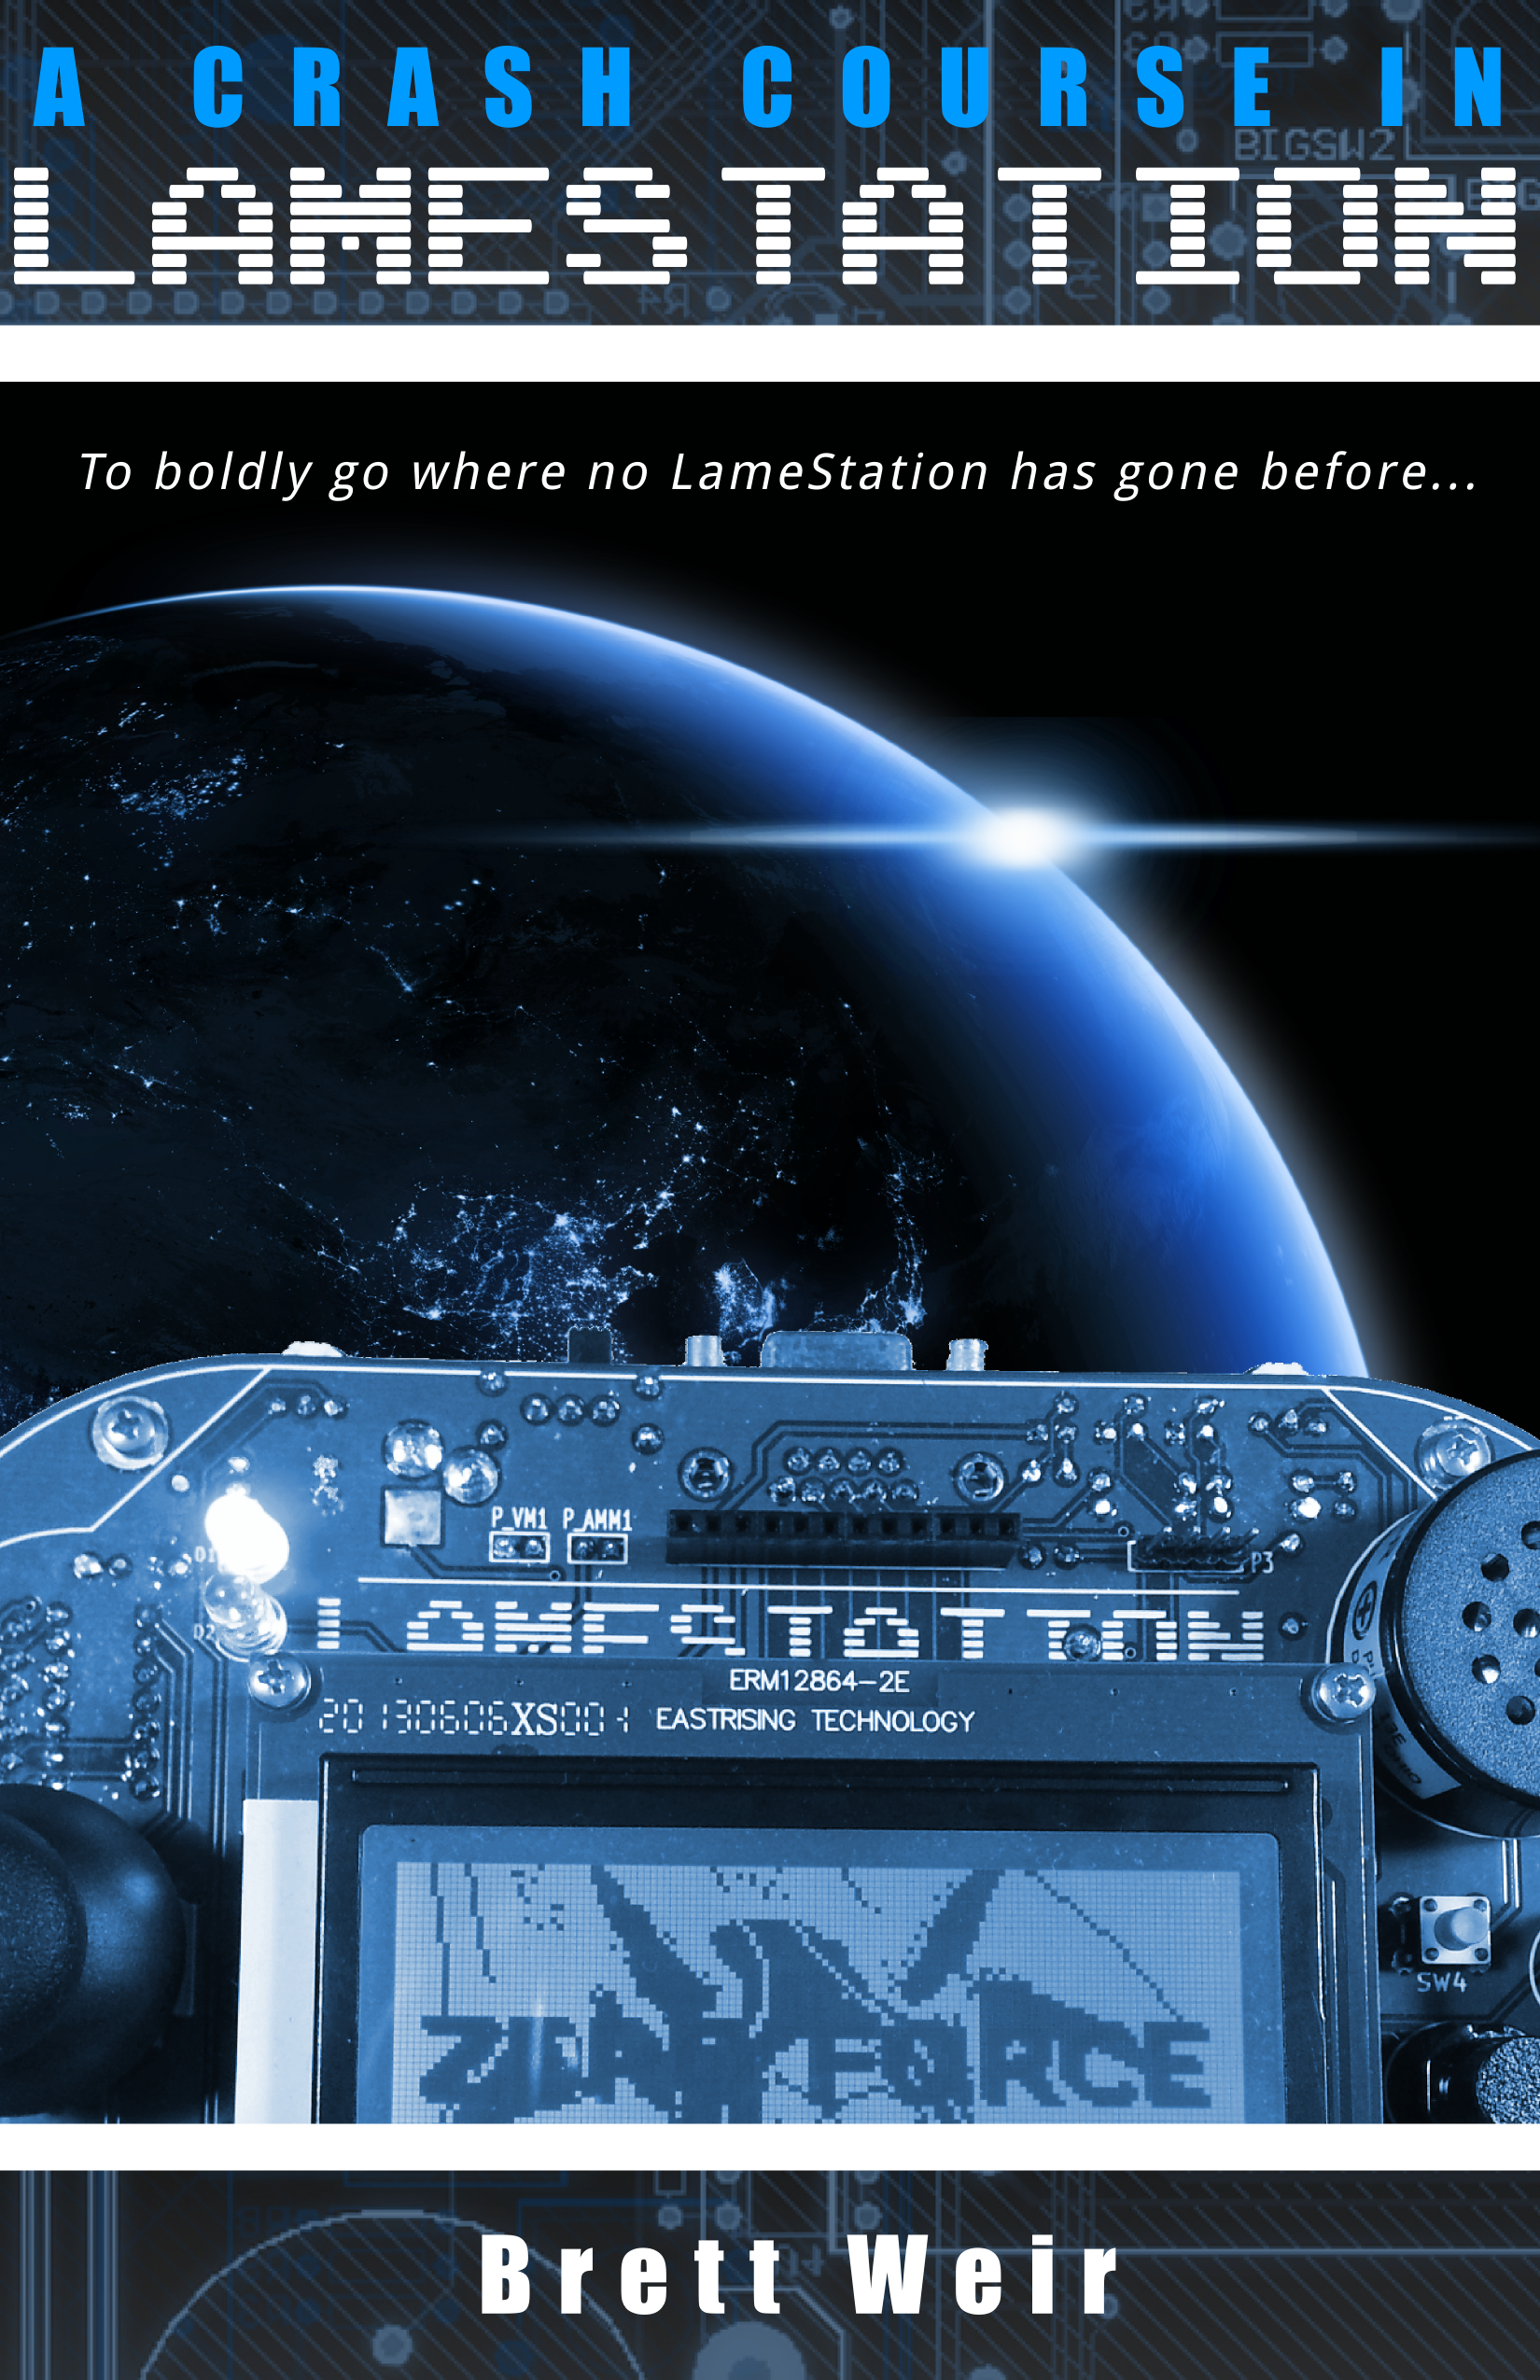
\includepdf{graphics/bookcover_front.png}
\cleardoublepage

		\newpage
														
\tableofcontents

\newpage



    \section{Abstract}

From a very young age, computers have been an integral part of my life.  I first discovered programming in the form of Graal Action Script, a language for developing non-player characters in an online game I enjoyed.  From there, I discovered DarkBASIC 3D game programming, then later in college, EECS 10 forced me to become acquainted with the wonderful world of C/C++ programming.  I began to develop my own video game, which would come to be known as piXel.  The game's concept was nothing original, but the thrill of seeing my ideas begin to take shape in a real and tangible form that I could show anyone ignited a fierce motivation within me to keep working.  

Video game development requires an intimate understanding of a wide array of concepts from a multitude of fields; engineering, computer science, mathematics, signal processing, physics, just to name a few.  And the development of a game console dually requires a broad swath of skills and background knowledge to develop such a device, which nominally includes power distribution, serial/parallel communications, digital audio synthesis and processing, human interface, video signal generation, PCB design and fabrication, and even networking.  A tremendous amount of effort over many tiresome nights has been put into the production of just such a device, and while not necessarily on par with the products manufactured by today's million-dollar research and development teams, the LameStation quite sufficiently showcases the many intricate facets of the development of such a device, and has proven an incredibly valuable experience in furthering my understanding of computer and electrical engineering.

It is my hope that after viewing the breadth and extent of the work required, even the most cynical of readers may come away with a greater appreciation for the magnificient feats of science and engineering inherent in each and every gaming device, and understand that they are far more than toys.

\begin{flushright}--Brett Weir\end{flushright}


\mainmatter

\part{Hardware}
\AddToShipoutPicture*{\ChapterBackgroundPic}
\clearpage

\chapter{Assembly}


    \section{Powering The Board}
\subsection{Parts Needed For This Section}

\begin{figure}[H]
		\centering
    \includegraphics[width = 2.5in]{attachments/9732135/9797698.jpg}\\
    \label{fig:zeldatwilight}
    \caption{\textcopyright  2006 Nintendo. \\ Note the luxurious resolution and detailed texture.}
\end{figure}

\begin{itemize}
\item
  1 x DC barrel jack
\item
  1 x Slide switch
\item
  1 x 5V regulator
\item
  1 x 3.3V regulator
\item
  3 x 100$\mu$F capacitors
\item
  1 x 4-pin socket
\item
  1 x Green LED
\item
  1 x 220$\Omega$ resistor
\item
  2 x Metric screw
\item
  2 x Metric nut
\end{itemize}

\subsection{Instructions}

The LameStation can be powered in one of two ways; using the on-board
4AAA battery pack or an external DC power supply. You do not need to
worry about conflicts between the two. The LS automatically switches
between the two sources using a shunt switch in the power jack. A
power-on LED is provided to prove, without a doubt, that the board is
actually on (you'll be happy to know, trust me).

The battery pack is a large, plastic obstruction to everything else you
need to assemble, so this is one of the last items to go on the board.
Instead, solder in the DC barrel jack for some unlimited power fun. Then
solder in the green LED and series resistor so that whenever you do
anything, you have a quick sanity check that the power has power at
least when troubleshooting.

Solder the DC barrel jack into \textbf{J1}. Do not solder in the
battery until later on. It's helpful for components like this to tape
or clip the component to the board before attempting to solder it.
That way it won't move around. I use electrical tape for this purpose.
You would also do well to get yourself a panoramic vise as it makes
soldering a million times easier.

Solder the large power switch into \textbf{SW1}.

Solder the 5V and 3.3V regulators into~\textbf{U2} and~\textbf{U3},
respectively. Bend them to be flat on the board. Do this before
installing the nearby capacitors or else it will be harder to get your
fingers around to bend it into place.

Solder 3 100$\mu$F capacitors into~\textbf{C3}, \textbf{C4}, and
\textbf{C5}. You'll want to leave a small amount of slack. These
capacitors are polarized, which means they have to be inserted in a
certain direction. You can determine the positive and negative
terminals by looking at the body of the capacitor. On the side of one
of the pins, you will find a strip of minus signs printed on the side.
This is the negative terminal. Now looking at the PCB, the capacitor's
footprint will have two holes, and one will have a plus sign. That
indicates the positive terminal, so make sure that the strip of minus
signs faces the other side, away from the `+' pad. Another pro tip: if
you have trouble getting the capacitor to stay on the board while
soldering, twist the leads around each other so that it will hold to
the board. You will just clip these off later, so you don't need to
worry about them touching so it's a nice fast way to get the component
to hold on.

Solder one of the 4-pin sockets into~\textbf{P4}. These pins provide
test points where you can
\href{Taking-Test-Measurements_9732196.html}{connect a voltmeter and
ammeter across the power supply} to take measurements.

Solder the green LED into~\textbf{D1} and a 220Ω resistor
into~\textbf{R24}. This will provide a power-on light to indicate when
the board is turned on, and is also an indicate of when there is a
short (if the power on but no light comes on).

This completes the power subsystem, except for the battery pack, which
will be connected later.

~

\begin{bclogo}[couleur=bgblue, arrondi =0 , logo=\bcbombe, barre=none,noborder=true]{Never blow up your LEDs again!}
\itshape The short lead wire on a capacitor or LED is the cathode, or negative terminal.
\end{bclogo}



Icon

\textbf{Watch That Green LED!}

The green LED does more than just tell you the board is on. It is also
an early warning system that you've done something horribly wrong. If
you've accidentally soldered something that has created a short in the
system, the green LED will not turn on, since no power can get to it.
\textbf{This may be the only warning you have}.

When you add a component, the first thing you should do when powering on
the board is watch that green LED. If it doesn't come on, \textbf{turn
off the power immediately}. This will reduce the chance of something
being fried on the board as a result of your mishap.

Icon

\textbf{Ground Connections}

You may have difficulty soldering connections that are wired to ground.
Just hold the iron to the pin longer until the solder flows.


								\newpage
\part{Software}
\AddToShipoutPicture*{\ChapterBackgroundPic}
\clearpage
\chapter{Display}
    \begin{itemize}
\itemsep1pt\parskip0pt\parsep0pt
\item
  \hyperref[LameAudio.spin-PublicFunctions]{Public Functions}
\item
  \hyperref[LameAudio.spin-PrivateFunctions]{Private Functions}
\end{itemize}

\hyperdef{}{LameAudio.spin-PublicFunctions}{\subsection{Public
Functions}\label{LameAudio.spin-PublicFunctions}}

\begin{itemize}
\itemsep1pt\parskip0pt\parsep0pt
\item
  \hyperref[LameAudio.spin-Start]{Start}
\item
  \hyperref[LameAudio.spin-SetADSR(attackvar,decayvar,sustainvar,releasevar)]{SetADSR(attackvar,
  decayvar, sustainvar, releasevar)}
\item
  \hyperref[LameAudio.spin-SetWaveform(waveformvar,volumevar)]{SetWaveform(waveformvar,
  volumevar)}
\item
  \hyperref[LameAudio.spin-LoadInstr(instrnum)]{LoadInstr(instrnum)}
\item
  \hyperref[LameAudio.spin-PlaySound(channel,note)]{PlaySound(channel,
  note)}
\item
  \hyperref[LameAudio.spin-StopSound(channel)]{StopSound(channel)}
\item
  \hyperref[LameAudio.spin-StopAllSound]{StopAllSound}
\item
  \hyperref[LameAudio.spin-PlaySequence(songAddrvar)]{PlaySequence(songAddrvar)}
\item
  \hyperref[LameAudio.spin-LoadSong(songBarAddrvar)]{LoadSong(songBarAddrvar)}
\item
  \hyperref[LameAudio.spin-PlaySong]{PlaySong}
\item
  \hyperref[LameAudio.spin-StopSong]{StopSong}
\item
  \hyperref[LameAudio.spin-SongPlaying]{SongPlaying}
\end{itemize}

\hyperdef{}{LameAudio.spin-Start}{\paragraph{Start}\label{LameAudio.spin-Start}}

\textbf{} ~Expand source

\lstset{style=spin}
\begin{lstlisting}
PUB Start
      
    parameter := @sine
    channelparam := (INITVAL << 8)
    channelADSR := LONG[@instruments][0]
    songchoice := SONGOFF
    looping := 0  
    play := 0
    
    
    repeat oscindexer from 0 to OSCREGS-1 step REGPEROSC
        oscRegister[oscindexer] := 0
        oscRegister[oscindexer+1] := 0
        oscRegister[oscindexer+2] := 0
        oscRegister[oscindexer+3] := 0
    oscindexer := 0
    oscindexcounter := 0
    
    cognew(@oscmodule, @parameter)    'start assembly cog
    cognew(LoopingSongParser, @LoopingPlayStack)
    
\end{lstlisting}

\hyperdef{}{LameAudio.spin-SetADSR(attackvar,decayvar,sustainvar,releasevar)}{\paragraph{SetADSR(attackvar,
decayvar, sustainvar,
releasevar)}\label{LameAudio.spin-SetADSR(attackvar,decayvar,sustainvar,releasevar)}}

\textbf{} ~Expand source

\lstset{style=spin}
\begin{lstlisting}
PUB SetADSR(attackvar, decayvar, sustainvar, releasevar)

    channelADSR := (channelADSR & A_MASK) + (attackvar << A_OFFSET)
    channelADSR := (channelADSR & D_MASK) + (decayvar << D_OFFSET)
    channelADSR := (channelADSR & S_MASK) + (sustainvar << S_OFFSET)
    channelADSR := (channelADSR & R_MASK) + (releasevar << R_OFFSET)
  
\end{lstlisting}

\hyperdef{}{LameAudio.spin-SetWaveform(waveformvar,volumevar)}{\paragraph{SetWaveform(waveformvar,
volumevar)}\label{LameAudio.spin-SetWaveform(waveformvar,volumevar)}}

\textbf{} ~Expand source

\lstset{style=spin}
\begin{lstlisting}
PUB SetWaveform(waveformvar, volumevar)

    channelADSR := (channelADSR & W_MASK) + (waveformvar << W_OFFSET)
    channelparam := (channelparam & $FFFF00FF) + (volumevar << 8)
\end{lstlisting}

\hyperdef{}{LameAudio.spin-LoadInstr(instrnum)}{\paragraph{LoadInstr(instrnum)}\label{LameAudio.spin-LoadInstr(instrnum)}}

\textbf{} ~Expand source

\lstset{style=spin}
\begin{lstlisting}
PUB LoadInstr(instrnum)

    channelADSR := LONG[@instruments][instrnum]
  
\end{lstlisting}

\hyperdef{}{LameAudio.spin-PlaySound(channel,note)}{\paragraph{PlaySound(channel,
note)}\label{LameAudio.spin-PlaySound(channel,note)}}

\textbf{} ~Expand source

\lstset{style=spin}
\begin{lstlisting}
PUB PlaySound(channel, note)

    if note < 128 and channel < VOICES
        oscindexer := channel << 2
        oscRegister[oscindexer] &= !KEYBITS          
        oscRegister[oscindexer+1] &= !ADSRBITS
        oscRegister[oscindexer] := note + KEYBITS
\end{lstlisting}

\hyperdef{}{LameAudio.spin-StopSound(channel)}{\paragraph{StopSound(channel)}\label{LameAudio.spin-StopSound(channel)}}

\textbf{} ~Expand source

\lstset{style=spin}
\begin{lstlisting}
PUB StopSound(channel)

    if channel < VOICES
        oscindexer := channel << 2          
        oscRegister[oscindexer] &= !KEYBITS 
\end{lstlisting}

\hyperdef{}{LameAudio.spin-StopAllSound}{\paragraph{StopAllSound}\label{LameAudio.spin-StopAllSound}}

\textbf{} ~Expand source

\lstset{style=spin}
\begin{lstlisting}
PUB StopAllSound

    repeat oscindexer from 0 to OSCREGS-1 step REGPEROSC
        oscRegister[oscindexer] &= !KEYBITS 
\end{lstlisting}

\hyperdef{}{LameAudio.spin-PlaySequence(songAddrvar)}{\paragraph{PlaySequence(songAddrvar)}\label{LameAudio.spin-PlaySequence(songAddrvar)}}

\textbf{} ~Expand source

\lstset{style=spin}
\begin{lstlisting}
PUB PlaySequence(songAddrvar)
    seqcursor := 0
    
    repeat while byte[songAddrvar][seqcursor] <> ENDOFSONG
        seqbyte := byte[songAddrvar][seqcursor]
        if seqbyte == TIMEWAIT
            repeatlong := byte[songAddrvar][seqcursor] << 13
            repeat repeatseqindex from 0 to repeatlong
            seqcursor += 2
        
        elseif seqbyte == NOTEON
            PlaySound(byte[songAddrvar][seqcursor+1],byte[songAddrvar][seqcursor+2])   
            seqcursor += 3
        
        elseif seqbyte == NOTEOFF
            StopSound(byte[songAddrvar][seqcursor+1])
            seqcursor += 2
\end{lstlisting}

\hyperdef{}{LameAudio.spin-LoadSong(songBarAddrvar)}{\paragraph{LoadSong(songBarAddrvar)}\label{LameAudio.spin-LoadSong(songBarAddrvar)}}

\textbf{} ~Expand source

\lstset{style=spin}
\begin{lstlisting}
PUB LoadSong(songBarAddrvar)

    barAddr := songBarAddrvar
    totalbars := byte[songBarAddrvar][0]
    repeatlong := byte[songBarAddrvar][1] << 8
    barres := byte[songBarAddrvar][2]
    loopsongPtr := barAddr + totalbars*(barres+BYTES_BARHEADER) + BYTES_SONGHEADER        
    
    songcursor := 0
    barcursor := 0
\end{lstlisting}

\hyperdef{}{LameAudio.spin-PlaySong}{\paragraph{PlaySong}\label{LameAudio.spin-PlaySong}}

\textbf{} ~Expand source

\lstset{style=spin}
\begin{lstlisting}
PUB PlaySong

    play := 1
\end{lstlisting}

\hyperdef{}{LameAudio.spin-StopSong}{\paragraph{StopSong}\label{LameAudio.spin-StopSong}}

\textbf{} ~Expand source

\lstset{style=spin}
\begin{lstlisting}
PUB StopSong

    play := 0
    StopAllSound
    
\end{lstlisting}

\hyperdef{}{LameAudio.spin-SongPlaying}{\paragraph{SongPlaying}\label{LameAudio.spin-SongPlaying}}

This function returns whether a song is currently playing

\textbf{} ~Expand source

\lstset{style=spin}
\begin{lstlisting}
PUB SongPlaying
    return play
        
\end{lstlisting}

\hyperdef{}{LameAudio.spin-PrivateFunctions}{\subsection{Private
Functions}\label{LameAudio.spin-PrivateFunctions}}

\begin{itemize}
\itemsep1pt\parskip0pt\parsep0pt
\item
  \hyperref[LameAudio.spin-FindLoopBarFromSongPointer]{FindLoopBarFromSongPointer}
\item
  \hyperref[LameAudio.spin-LoopingSongParser]{LoopingSongParser}
\end{itemize}

\hyperdef{}{LameAudio.spin-FindLoopBarFromSongPointer}{\paragraph{FindLoopBarFromSongPointer}\label{LameAudio.spin-FindLoopBarFromSongPointer}}

This function increments the loop pointer by the value of the song
pointr

\textbf{} ~Expand source

\lstset{style=spin}
\begin{lstlisting}
PRI FindLoopBarFromSongPointer

    barinc := 0
    barshift := 0
    repeat while barinc < byte[loopsongPtr][songcursor]
        barshift += barres+BYTES_BARHEADER
        barinc++
\end{lstlisting}

\hyperdef{}{LameAudio.spin-LoopingSongParser}{\paragraph{LoopingSongParser}\label{LameAudio.spin-LoopingSongParser}}

\textbf{} ~Expand source

\lstset{style=spin}
\begin{lstlisting}
PRI LoopingSongParser

    repeat

        if play == 1
            songcursor := 0
               
            ' iterate through song definition lines
            repeat while byte[loopsongPtr][songcursor] <> SONGOFF and play == 1  
                
                barcursor := songcursor
                
                
                ' iterate through loop definitions
                repeat linecursor from 0 to (barres-1)
                
                    songcursor := barcursor

                    ' play all notes defined in song definition
                    repeat while byte[loopsongPtr][songcursor] <> BAROFF and play == 1  
                        FindLoopBarFromSongPointer 
                        
                        bartmp := barshift+BYTES_SONGHEADER+BYTES_BARHEADER+linecursor
                        
                        if byte[barAddr][bartmp] == SNOP

                        elseif byte[barAddr][bartmp] == SOFF
                            StopSound( byte[barAddr][barshift+BYTES_SONGHEADER] )       
                            
                        else
                            PlaySound( byte[barAddr][barshift+BYTES_SONGHEADER] , byte[barAddr][bartmp] )  'channel, note

                            
                        songcursor += 1
                    
                    repeat repeatindex from 0 to repeatlong
                   
                songcursor += 1

            StopAllSound
\end{lstlisting}

    \newpage
\section{Blitting Operations}



\subsection*{Screen Clear}

This command arbitrarily clears the screen buffer to black and requires no parameters.  It does not access any memory additional to the buffer itself.

\lstset{style=pasm}
\begin{lstlisting}
clearscreen1            mov     Addrtemp, destscrn
                        mov     valutemp, fulscreen
       
:loop                   mov     datatemp, Addrtemp
                        add     datatemp, frmflipcurrent
                        wrword  zero, datatemp
                        add     Addrtemp, #2
                        djnz    valutemp, #:loop
                        jmp     #loopexit
\end{lstlisting}





\subsection*{Screen Blit}

This command copies a screen-sized memory block into the screen buffer.  It is the simplest form of blitting as no knowledge of the image's on-screen location is required; only knowledge that the source image is the same size as the destination buffer.

\begin{lstlisting}
blitscreen1             mov     Addrtemp, destscrn
                        rdlong  Addrtemp2, sourceAddr
                        mov     valutemp, fulscreen
       
:loop                   mov     datatemp, Addrtemp
                        add     datatemp, frmflipcurrent
           
                        rdword  datatemp2, Addrtemp2
                        wrword  datatemp2, datatemp
                        add     Addrtemp, #2
                        add     Addrtemp2, #2
                        djnz    valutemp, #:loop
                        jmp     #loopexit
\end{lstlisting}





\subsection*{Box Blit}

This command copies a square image with a width of 8 pixels to the screen.  It is the simplest function for drawing tiled levels to the screen, as it requires only position and source data as an input.  However, vertical position is limited by the position problem, and care must be taken not to draw into inappropriate regions of memory, as memory corruption may occur.




\subsection*{Sprite Blit}

Sprite blit is a more sophisticated drawing routine that allows for arbitrary positioning on the screen, arbitrary image dimensions, and ensures images are not drawn outside the appropriate areas of the screen.  This additional functionality comes at a computational price, but efficiently use of resources can enable the user to create more dynamic games than otherwise.





\subsection*{Masked Sprite Blit}

This function takes sprite blitting one step further.  It allows the user to key out certain regions of an image that would otherwise be copied, allowing an image to be drawn seamlessly onto a backdrop, even if it is not of a rectangular shape.  This is a problem experienced by, for example, a ball sprite.  Without keying, the ball is drawn with its bounding box, appearing unsightly and out of place.  With keying, the ball is just another part of the scene.

\begin{figure}[H]
	\centering
	
		\begin{tabular} {c c | c}
		Flip & Color & Mask bit \\
		\hline
		0 & 0 & 0 \\
		0 & 1 & 0 \\
		1 & 0 & 1 \\
		1 & 1 & 0 \\
		\end{tabular}
		
	\label{maskblittruthtable}
	\caption{Truth Table}

\end{figure}

This operation is equivalent to Mask = Flip ANDN Color.


\lstset{style=C++}

\newpage
\section{Frequencytiming}


%\section{Specifications}

%						\input{specs/specifications.tex}
%								\newpage				
								
								
																			
%\section{The Microcontroller}
%
%						\input{proppa/proppa.tex}	
%								\newpage
%
%\section{Display}
%%						\input{display/schem.tex}
%						\input{display/intro.tex}
%						\input{display/whymono.tex}
%					 	\input{display/driver.tex}						
%
%					 	\newpage
\section{Blitting Operations}



\subsection*{Screen Clear}

This command arbitrarily clears the screen buffer to black and requires no parameters.  It does not access any memory additional to the buffer itself.

\lstset{style=pasm}
\begin{lstlisting}
clearscreen1            mov     Addrtemp, destscrn
                        mov     valutemp, fulscreen
       
:loop                   mov     datatemp, Addrtemp
                        add     datatemp, frmflipcurrent
                        wrword  zero, datatemp
                        add     Addrtemp, #2
                        djnz    valutemp, #:loop
                        jmp     #loopexit
\end{lstlisting}





\subsection*{Screen Blit}

This command copies a screen-sized memory block into the screen buffer.  It is the simplest form of blitting as no knowledge of the image's on-screen location is required; only knowledge that the source image is the same size as the destination buffer.

\begin{lstlisting}
blitscreen1             mov     Addrtemp, destscrn
                        rdlong  Addrtemp2, sourceAddr
                        mov     valutemp, fulscreen
       
:loop                   mov     datatemp, Addrtemp
                        add     datatemp, frmflipcurrent
           
                        rdword  datatemp2, Addrtemp2
                        wrword  datatemp2, datatemp
                        add     Addrtemp, #2
                        add     Addrtemp2, #2
                        djnz    valutemp, #:loop
                        jmp     #loopexit
\end{lstlisting}





\subsection*{Box Blit}

This command copies a square image with a width of 8 pixels to the screen.  It is the simplest function for drawing tiled levels to the screen, as it requires only position and source data as an input.  However, vertical position is limited by the position problem, and care must be taken not to draw into inappropriate regions of memory, as memory corruption may occur.




\subsection*{Sprite Blit}

Sprite blit is a more sophisticated drawing routine that allows for arbitrary positioning on the screen, arbitrary image dimensions, and ensures images are not drawn outside the appropriate areas of the screen.  This additional functionality comes at a computational price, but efficiently use of resources can enable the user to create more dynamic games than otherwise.





\subsection*{Masked Sprite Blit}

This function takes sprite blitting one step further.  It allows the user to key out certain regions of an image that would otherwise be copied, allowing an image to be drawn seamlessly onto a backdrop, even if it is not of a rectangular shape.  This is a problem experienced by, for example, a ball sprite.  Without keying, the ball is drawn with its bounding box, appearing unsightly and out of place.  With keying, the ball is just another part of the scene.

\begin{figure}[H]
	\centering
	
		\begin{tabular} {c c | c}
		Flip & Color & Mask bit \\
		\hline
		0 & 0 & 0 \\
		0 & 1 & 0 \\
		1 & 0 & 1 \\
		1 & 1 & 0 \\
		\end{tabular}
		
	\label{maskblittruthtable}
	\caption{Truth Table}

\end{figure}

This operation is equivalent to Mask = Flip ANDN Color.


\lstset{style=C++}

%
%						\input{display/contentgeneration.tex}												
%								\newpage												
%												
%												
%\section{Audio}
%%						\input{audio/schem.tex}
%
%						\input{support/allegfuncgen.tex}
%						\input{support/mathfuncgen.tex}
%
%						\input{support/wav2dat.tex}
%						\input{support/frequencytablegenerator.tex}
%
%						\input{audio/frequencytiming.tex}
%						%\input{../cprograms/frequencytable_latex.txt}
%						\input{audio/frequencytiming/propellertiming.tex}
%			
%						\input{audio/phaseaccumulator.tex}
%						\input{audio/typesofsound.tex}
%								\newpage					
%								
%					  \input{audio/asm_spin_interface.tex}
%						\input{audio/pwm_dac.tex}
%
%								\newpage
%
%\section{Power}
%%						\input{power/schem.tex}
%						\input{power/consumption.tex}
%
%								\newpage
%
%
%
%\section{Controls}
%%						\input{controls/schem.tex}
%						\input{controls/joystick.tex}
%						\input{controls/buttons.tex}
%
%								\newpage
%
%%\section{Utilities}
%
%%						\input{support/intro.tex}
%
%
%
%\section{Constraints}
%						\input{constraints/sustainability.tex}
%
%
%
%\section{Applications}
%%						\input{apps/schem.tex}
%						\input{apps/midi_interfacing.tex}
%						\input{apps/wireless.tex}
%
%						\newpage
%
%
%%\section{Source}
%				%		\input{specs/source.tex}
%
%
%
%
%

\backmatter
    \printindex

\end{document}
